\lstinputlisting[language=C++]{solutions/loop_unrolling/factor4/fir_loop_unrolling_manual_factor4.cpp}
\lstinputlisting[language=C++]{solutions/loop_unrolling/factor4/fir_loop_unrolling_automatic_factor4.cpp}
\lstinputlisting[language=C++]{solutions/loop_unrolling/factor4/fir_loop_unrolling_automatic_partiotioning_factor4.cpp}

\begin{table}[H]
    \centering
    \begin{tabular}{|c|c|c|c|c|}
        \hline
        \textbf{Solution} & \textbf{Clock} & \textbf{Target} & \textbf{Estimated} & \textbf{Uncertainty} \\
        \hline
        Manuale & ap\_clk & 10.00 & 8.510 & 1.25 \\
        \hline
        Automatico & ap\_clk & 10.00 & 8.510 & 1.25 \\
        \hline
        Automatico con Partitioning & ap\_clk & 10.00 & 8.510 & 1.25 \\
        \hline
    \end{tabular}
    \caption{HLS Loop Unrolling Factor=4 Solution Timing Summary (ns)}
    \label{tab:hls-loop-unrolling-factor4-solution-timing-summary}
\end{table}

\begin{table}[H]
    \centering
    \begin{tabular}{|c|c|c|c|c|}
        \hline
        \multicolumn{1}{|c|}{\textbf{Solution}} & \multicolumn{2}{|c|}{\textbf{Latency}} & \multicolumn{2}{|c|}{\textbf{Interval}} \\
        & min & max & min & max \\
        \hline
        Manuale & 58 & 58 & 58 & 58 \\
        \hline
        Automatico & 62 & 66 & 62 & 66 \\
        \hline
        Automatico con Partitioning & 62 & 64 & 62 & 64 \\
        \hline
    \end{tabular}
    \caption{HLS Loop Unrolling Factor=4 Solution Latency Summary (clock cycles)}
    \label{tab:hls-loop-unrolling-factor4-solution-latency-summary}
\end{table}

\begin{table}[H]
    \centering
    \begin{tabular}{|c|c|c|c|c|c|c|c|c|c|}
        \hline
        \multicolumn{1}{|c|}{\textbf{Solution}} & \multicolumn{1}{|c|}{Loop Name} & \multicolumn{2}{|c|}{\textbf{Latency}} & \multicolumn{2}{c|}{\textbf{Iteration Latency}} & \multicolumn{2}{c|}{\textbf{Initiation Interval}} & \multicolumn{1}{c|}{\textbf{Trip}}  \\
        &  & min & max & min & max & achieved & target & \textbf{Count} \\
        \hline
        Manuale & - loopShifting & 12 & 12 & 4 & 4 & - & - & 3 \\
        & - loopAccumulator & 44 & 44 & 4 & 4 & - & - & 11 \\
        \hline
        Automatico & - loopShifting & 15 & 18 & 5 & 5 & - & - & 3 \\
        & - loopAccumulator & 44 & 44 & 4 & 4 & - & - & 11 \\
        \hline
        Automatico  & - loopShifting & 15 & 17 & 5 & 5 & - & - & 3 \\
        con Partitioning & - loopAccumulator & 44 & 44 & 4 & 4 & - & - & 11 \\
        \hline
    \end{tabular}
    \caption{HLS Loop Unrolling Factor=4 Solution Latency Loops Summary }
    \label{tab:hls-loop-unrolling-factor4-solution-loop-summary}
\end{table}

In questo caso si può notare come il trip count sia, ovviamente, il medesimo per tutte e tre le soluzioni. Ciò che cambia effettivamente, come nel caso del fattore pari a 2, è la latency associata ai loop. In particolare, analizzando più nel dettaglio, tramite l'interfaccia Analysis, si può evidenziare come il loopShifting, in cui viene implementato un parallelismo pari a 4, viene gestito in maniera differente. Infatti, nel caso del loop unrolling manuale, vengono effettuate in parallelo due read alla volta e poi successivamente vengono eseguite in parallelo due write alla volta. Invece, nel caso della soluzione hardware basata su unrolling automatico, vengono effettuate una read e una write in parallelo per ogni ciclo di latenza. Nello specifico, considerando quattro shifting per ogni iterazione, viene effettuata la read al primo ciclo di latenza e, successivamente, viene eseguita la write corrispondente in parallelo alla read relativo al secondo shifting e così via. Di conseguenza, si avranno cinque colpi di latenza per ogni iterazione come riportato dal valore di iteration latency del report di sintesi.

\begin{figure}[H]
    \centering
    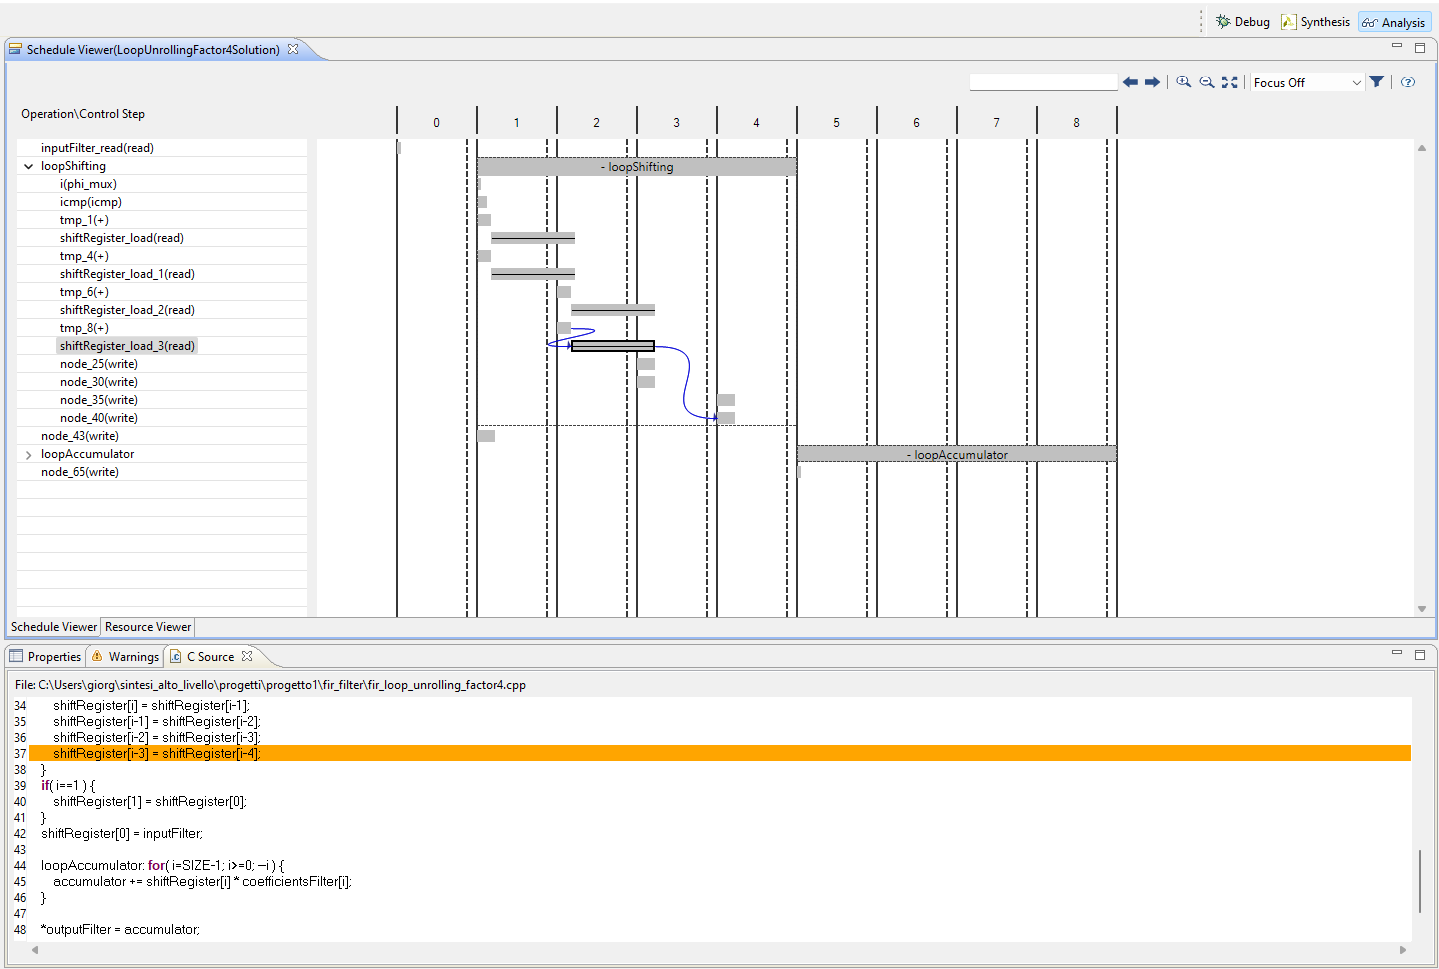
\includegraphics[width=0.9\textwidth]{solutions/loop_unrolling/factor4/loopunrollingmanual4.png}
    \caption{HLS Loop Unrolling Manual Factor=4 Analysis}
\end{figure}

\begin{figure}[H]
    \centering
    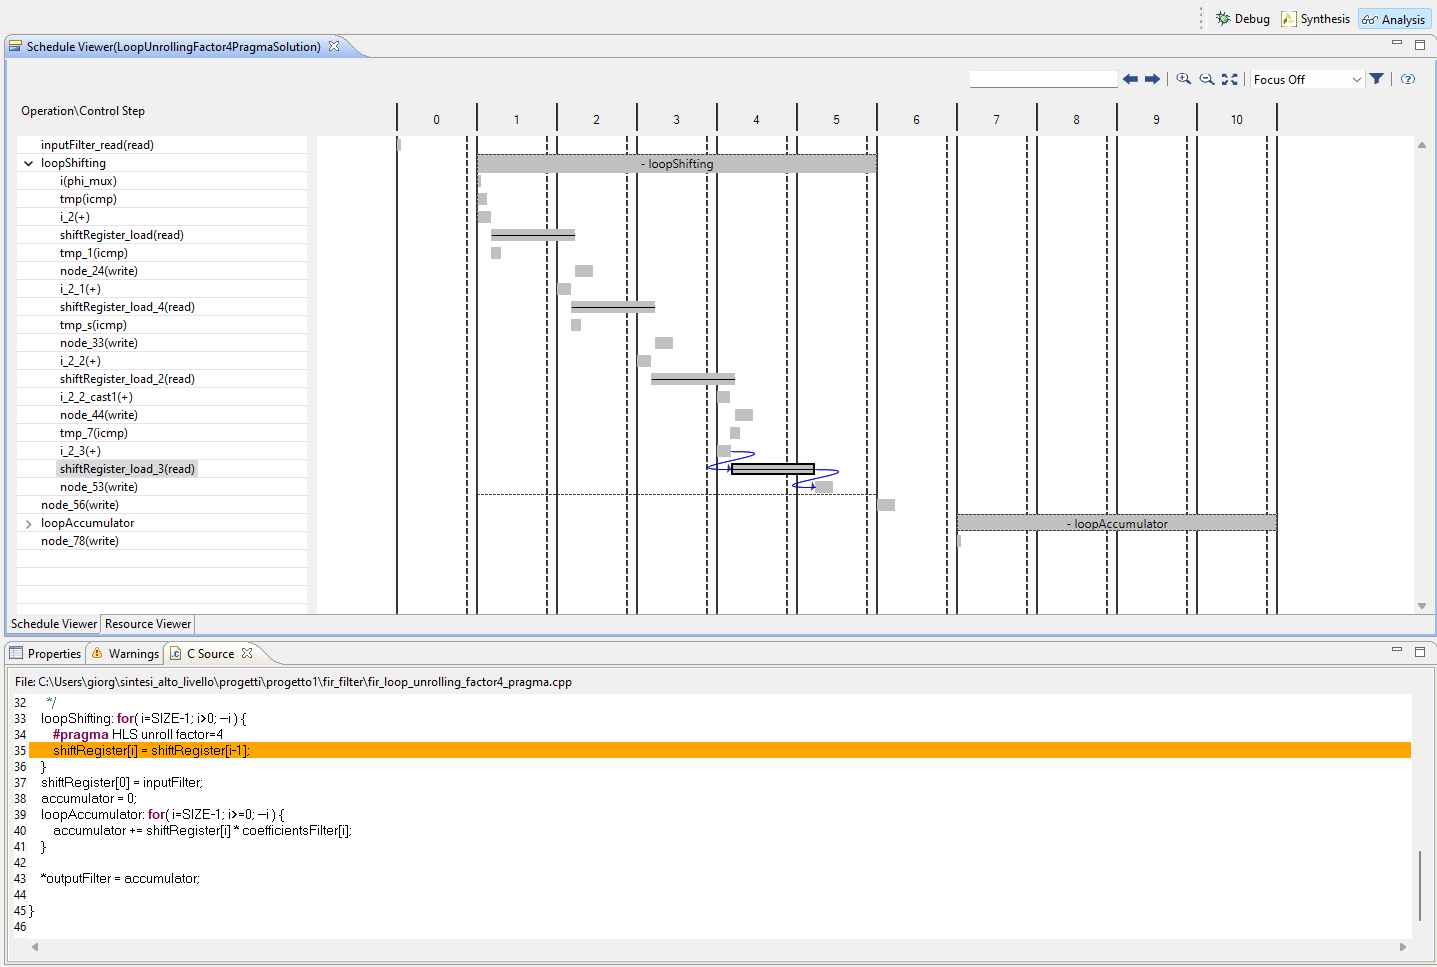
\includegraphics[width=0.9\textwidth]{solutions/loop_unrolling/factor4/loopunrollingautomatic4.png}
    \caption{HLS Loop Unrolling Automatic Factor=4 Analysis}
\end{figure}

Analogamente a quanto è stato analizzato e descritto nel caso di parallelismo di fattore pari a 2, anche in questo caso si può notare come l'utilizzazione delle risorse sia quasi la medesima tra il loop unrolling manuale e automatico. Invece, per quanto riguarda il loop unrolling automatico con partitioning, si ha un notevole aumento dell'utilizzazione sia di FF sia di LUT.

\begin{table}[H]
    \centering
    \begin{tabular}{|c|c|c|c|c|}
        \hline
        \textbf{Solution} & \textbf{BRAM\_18K} & \textbf{DSP48E} & \textbf{FF} & \textbf{LUT} \\
        \hline
        Manuale & 2 & 2 & 221 & 318 \\
        \hline
        Automatico & 2 & 2 & 194 & 367 \\
        \hline
        Automatico con Partitioning & 0 & 2 & 928 & 748 \\
        \hline
    \end{tabular}
    \caption{HLS Loop Unrolling Factor=4 Solution Utilization Estimates [\#]}
    \label{tab:vivado-loop-unrolling-factor4-solution-utilization-report}
\end{table}

Qui di seguito vengono riportati i report relativi alla C/RTL Cosimulation, dove è possibile analizzare il numero di cicli di clock che servono per ottenere un risultato in uscita, e quello relativo a Export RTL.

\begin{table}[H]
    \centering
    \begin{tabular}{|c|c|c|c|c|c|c|c|c|}
        \hline
        \multicolumn{1}{|c|}{\textbf{Solution}} & \multicolumn{1}{|c|}{RTL} & \multicolumn{1}{|c|}{Status} & \multicolumn{3}{c|}{\textbf{Latency}} & \multicolumn{3}{c|}{\textbf{Interval}} \\
        & &  & min & avg & max & min & avg & max \\
        \hline
        Manuale & VHDL & Pass & 58 & 58 & 59 & 58 & 58 & 59 \\
        \hline
        Automatico & VHDL & Pass & 60 & 60 & 61 & 60 & 60 & 61 \\
        \hline
        Automatico con Partitioning & VHDL & Pass & 58 & 58 & 59 & 58 & 58 & 59 \\
        \hline
    \end{tabular}
    \caption{HLS Loop Unrolling Factor=4 Solution C/RTL Cosimulation Report }
    \label{tab:hls-loop-unrolling-factor4-solution-cosimulation-report}
\end{table}

\begin{table}[H]
    \centering
    \begin{tabular}{|c|c|c|c|c|c|c|c|c|}
        \hline
        \textbf{Solution} & \textbf{SLICE} & \textbf{LUT} & \textbf{FF} & \textbf{DSP} & \textbf{BRAM} & \textbf{CP} & \textbf{CP} & \textbf{CP} \\
        & & & & & & \textbf{required} & \textbf{achieved} & \textbf{achieved}\\
        & & & & & & & \textbf{post-} & \textbf{post-}\\
        & & & & & & & \textbf{synthesis} & \textbf{implementation}\\
        \hline
        Manuale & 46 & 160 & 147 & 2 & 2 & 10 & 5.745 & 5.692 \\
        \hline
        Automatico & 40 & 145 & 93 & 2 & 2 & 10 & 5.745 & 5.692 \\
        \hline
        Automatico  & 412 & 1145 & 864 & 2 & 0 & 10 & 5.745 & 7.109 \\
        con Partitioning & & & & & & & & \\
        \hline
    \end{tabular}
    \caption{HLS Loop Unrolling Factor=4 Solution Export RTL Report}
    \label{tab:vivado-loop-unrolling-factor4-solution-export-rtl-report}
\end{table}

Pertanto, importando l'IP in Vivado e impostando un clock constraint pari a 10ns è possibile analizzare i seguenti report di risorse, timing, potenza dinamica ed energia per singola operazione.
\lstinputlisting[language=VHDL]{solutions/loop_unrolling/factor2/clk_constraint.xdc}

Analogamente all'unrolling di fattore pari a 2, anche in questo caso in corrispondenza della soluzione hardware basata su unrolling e partizionamento si ha un notevole aumento di utilizzazione delle risorse. Inoltre, si può notare come il numero di FF utilizzati per la solution di unrolling automatico risulta essere circa il $37\%$ in meno rispetto a quella basata su unrolling manuale. Evidentemente il tool, tramite la direttiva proprietaria, è riuscito ad effettuare delle ottimizzazione tali da garantire una diminuzione dei Flip Flop.

\begin{table}[H]
    \centering
    \begin{tabular}{|c|c|c|c|c|c|c|c|}
        \hline
        \textbf{Solution} & \textbf{LUT} & \textbf{LUTRAM} & \textbf{FF} & \textbf{BRAM} & \textbf{DSP} & \textbf{IO} & \textbf{BUFG} \\
        \hline
        Manuale & 159 & 0 & 147 & 1 & 2 & 71 & 1 \\
        \hline
        Automatico & 145 & 0 & 93 & 1 & 2 & 71 & 1 \\
        \hline
        Automatico & 1145 & 0 & 864 & 0 & 2 & 71 & 1 \\
        con Partitioning & & & & & & & \\
        \hline
    \end{tabular}
    \caption{Vivado Loop Unrolling Factor=4 Solution Utilization Report [\#]}
    \label{tab:vivado-loop-unrolling-factor4-utilization-report}
\end{table}

Effettuando un confronto grafico e tenendo conto dei dati precedentemente ottenuti per la soluzione basata su scissione del loop, si può notare come l'utilizzazione delle risorse sia pressocché la medesima tra loop fission e loop unrolling automatico.

\begin{figure}[H]
    \centering
    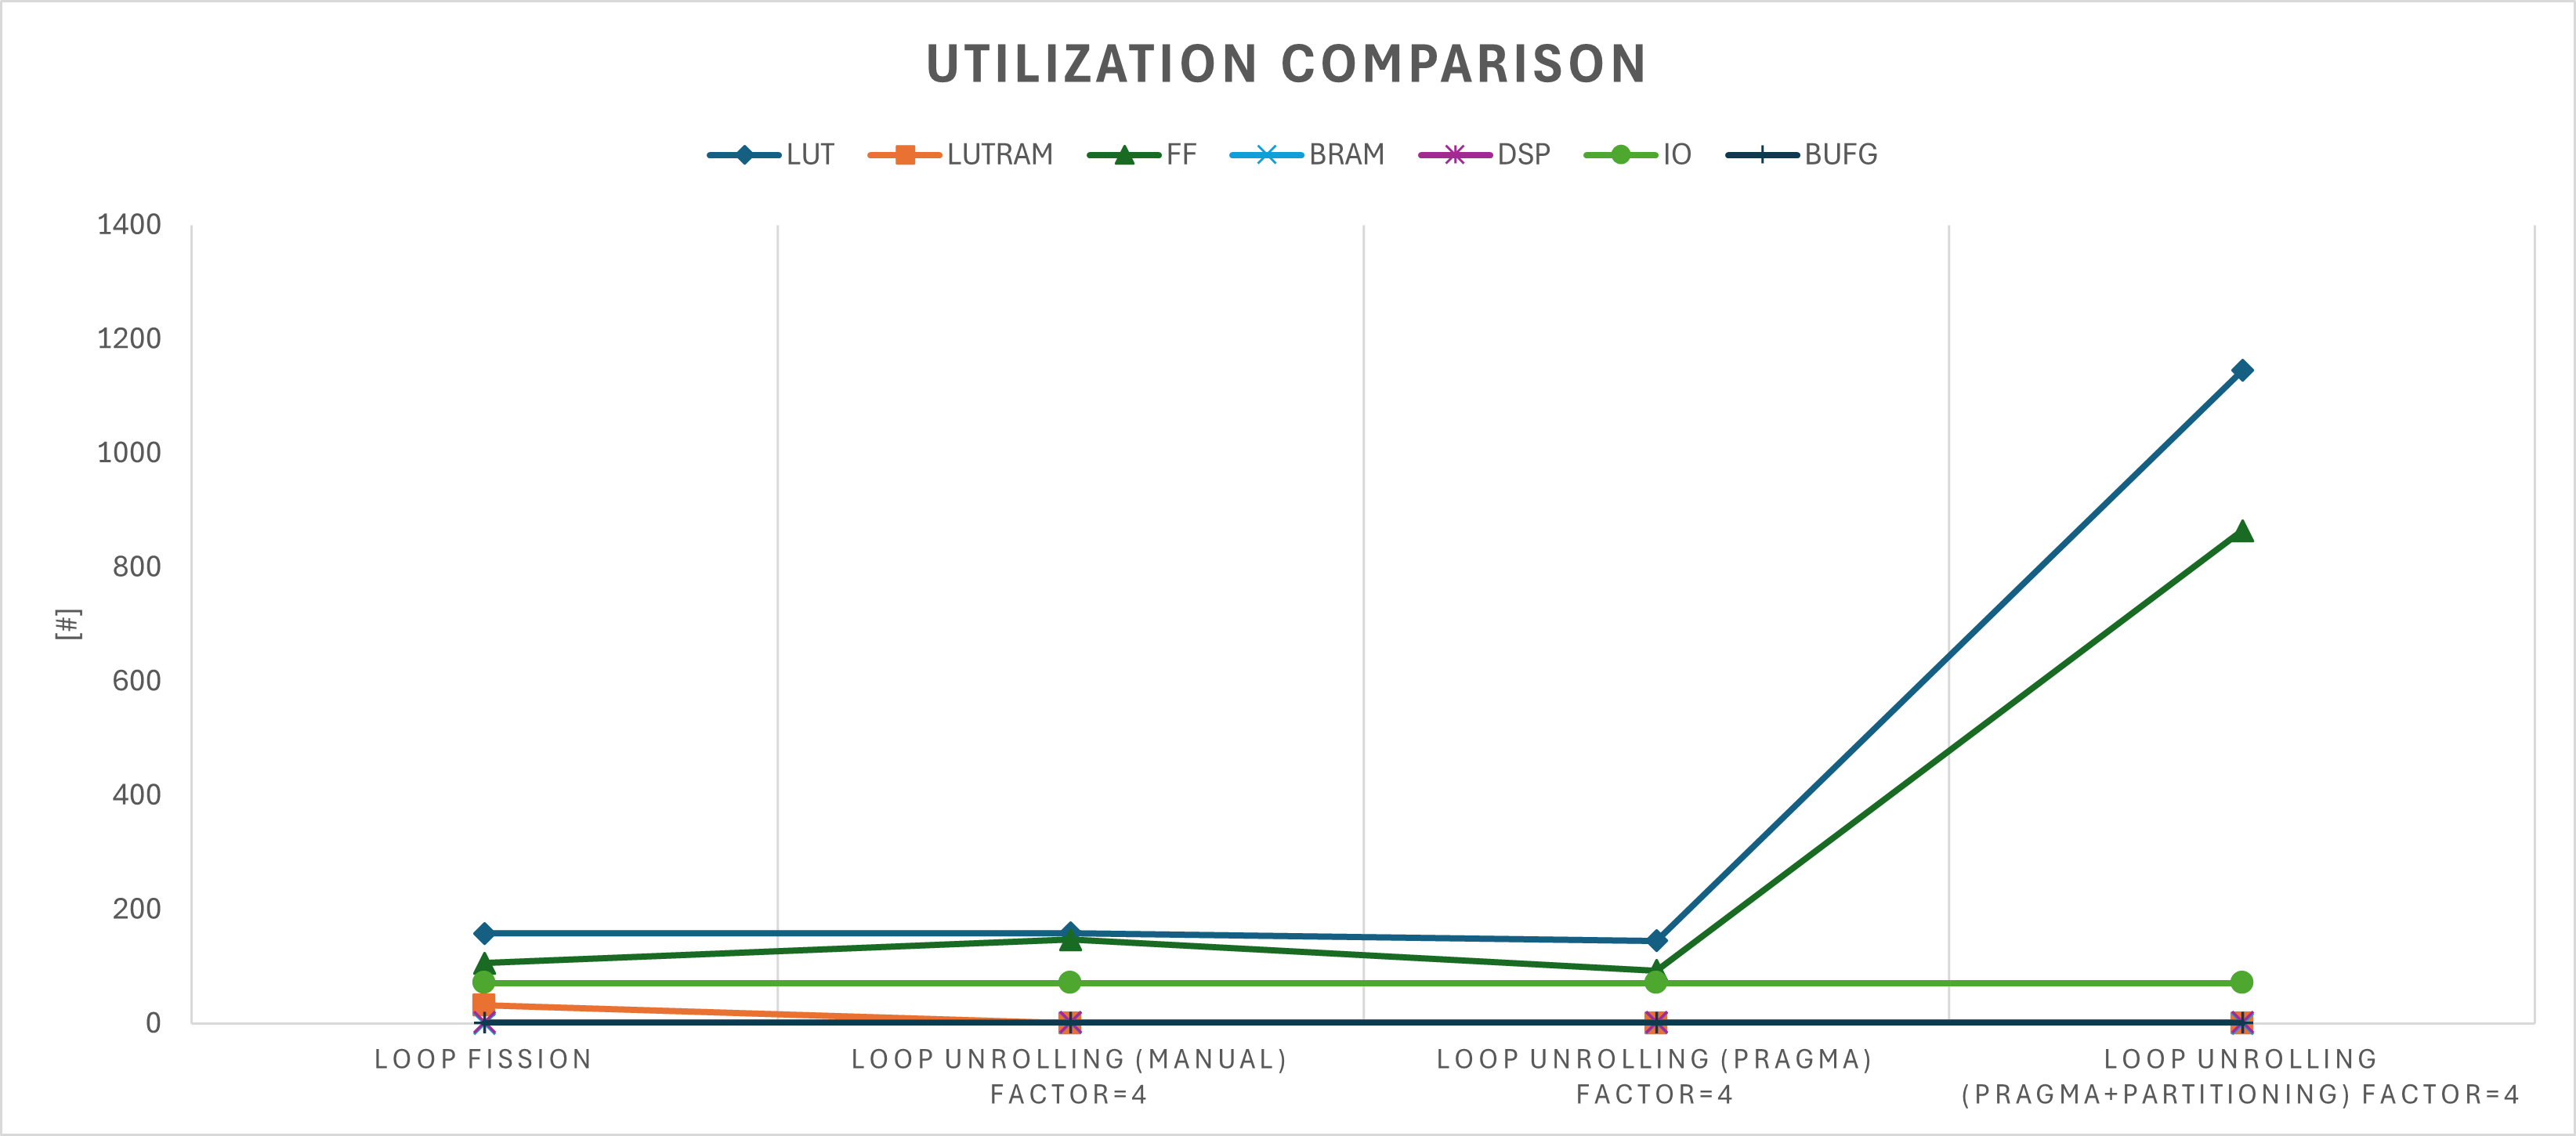
\includegraphics[width=0.9\textwidth]{solutions/loop_unrolling/factor4/loopunrollingfactor4utilization.png}
    \caption{Vivado Loop Unrolling Factor=4 Utilization Plot}
    \label{fig:vivado-loop-unrolling-factor4-utilization-plot}
\end{figure}

Per quanto riguarda il report di timing, è possibile notare, analogamente a quanto successo per l'unrolling di fattore pari a 2, una diminuzione della maximum clock frequency in corrispondenza della soluzione basata su loop unrolling automatico con partizionamento.

\begin{table}[H]
    \centering
    \begin{tabular}{|c|c|c|c|c|}
        \hline
        \textbf{Solution} & \textbf{Cycles} [\#] & \textbf{Clock Constraint} [ns] & \textbf{WNS} [ns] & \textbf{Maximum Clock} \\
        & & & & \textbf{Frequency} [MHz] \\
        \hline
        Manuale & 59 & 10 & 4.257 & 174.1250218 \\
        \hline
        Automatico & 61 & 10 & 4.33 & 176.366843 \\
        \hline
        Automatico & 59 & 10 & 3.097 & 144.8645516 \\
        con Partitioning & & & & \\
        \hline
    \end{tabular}
    \caption{Vivado Loop Unrolling Factor=4 Solution Timing Report}
    \label{tab:vivado-loop-unrolling-factor4-solution-timing-report}
\end{table}

Per quanto riguarda, invece, il numero di cicli di clock per garantire un risultato in uscita, in questo caso, per le tre soluzioni basate su unrolling di fattore pari a 4, si è ottenuto un valore minore rispetto alla soluzione basata su scissione del loop. 

\begin{figure}[H]
    \centering
    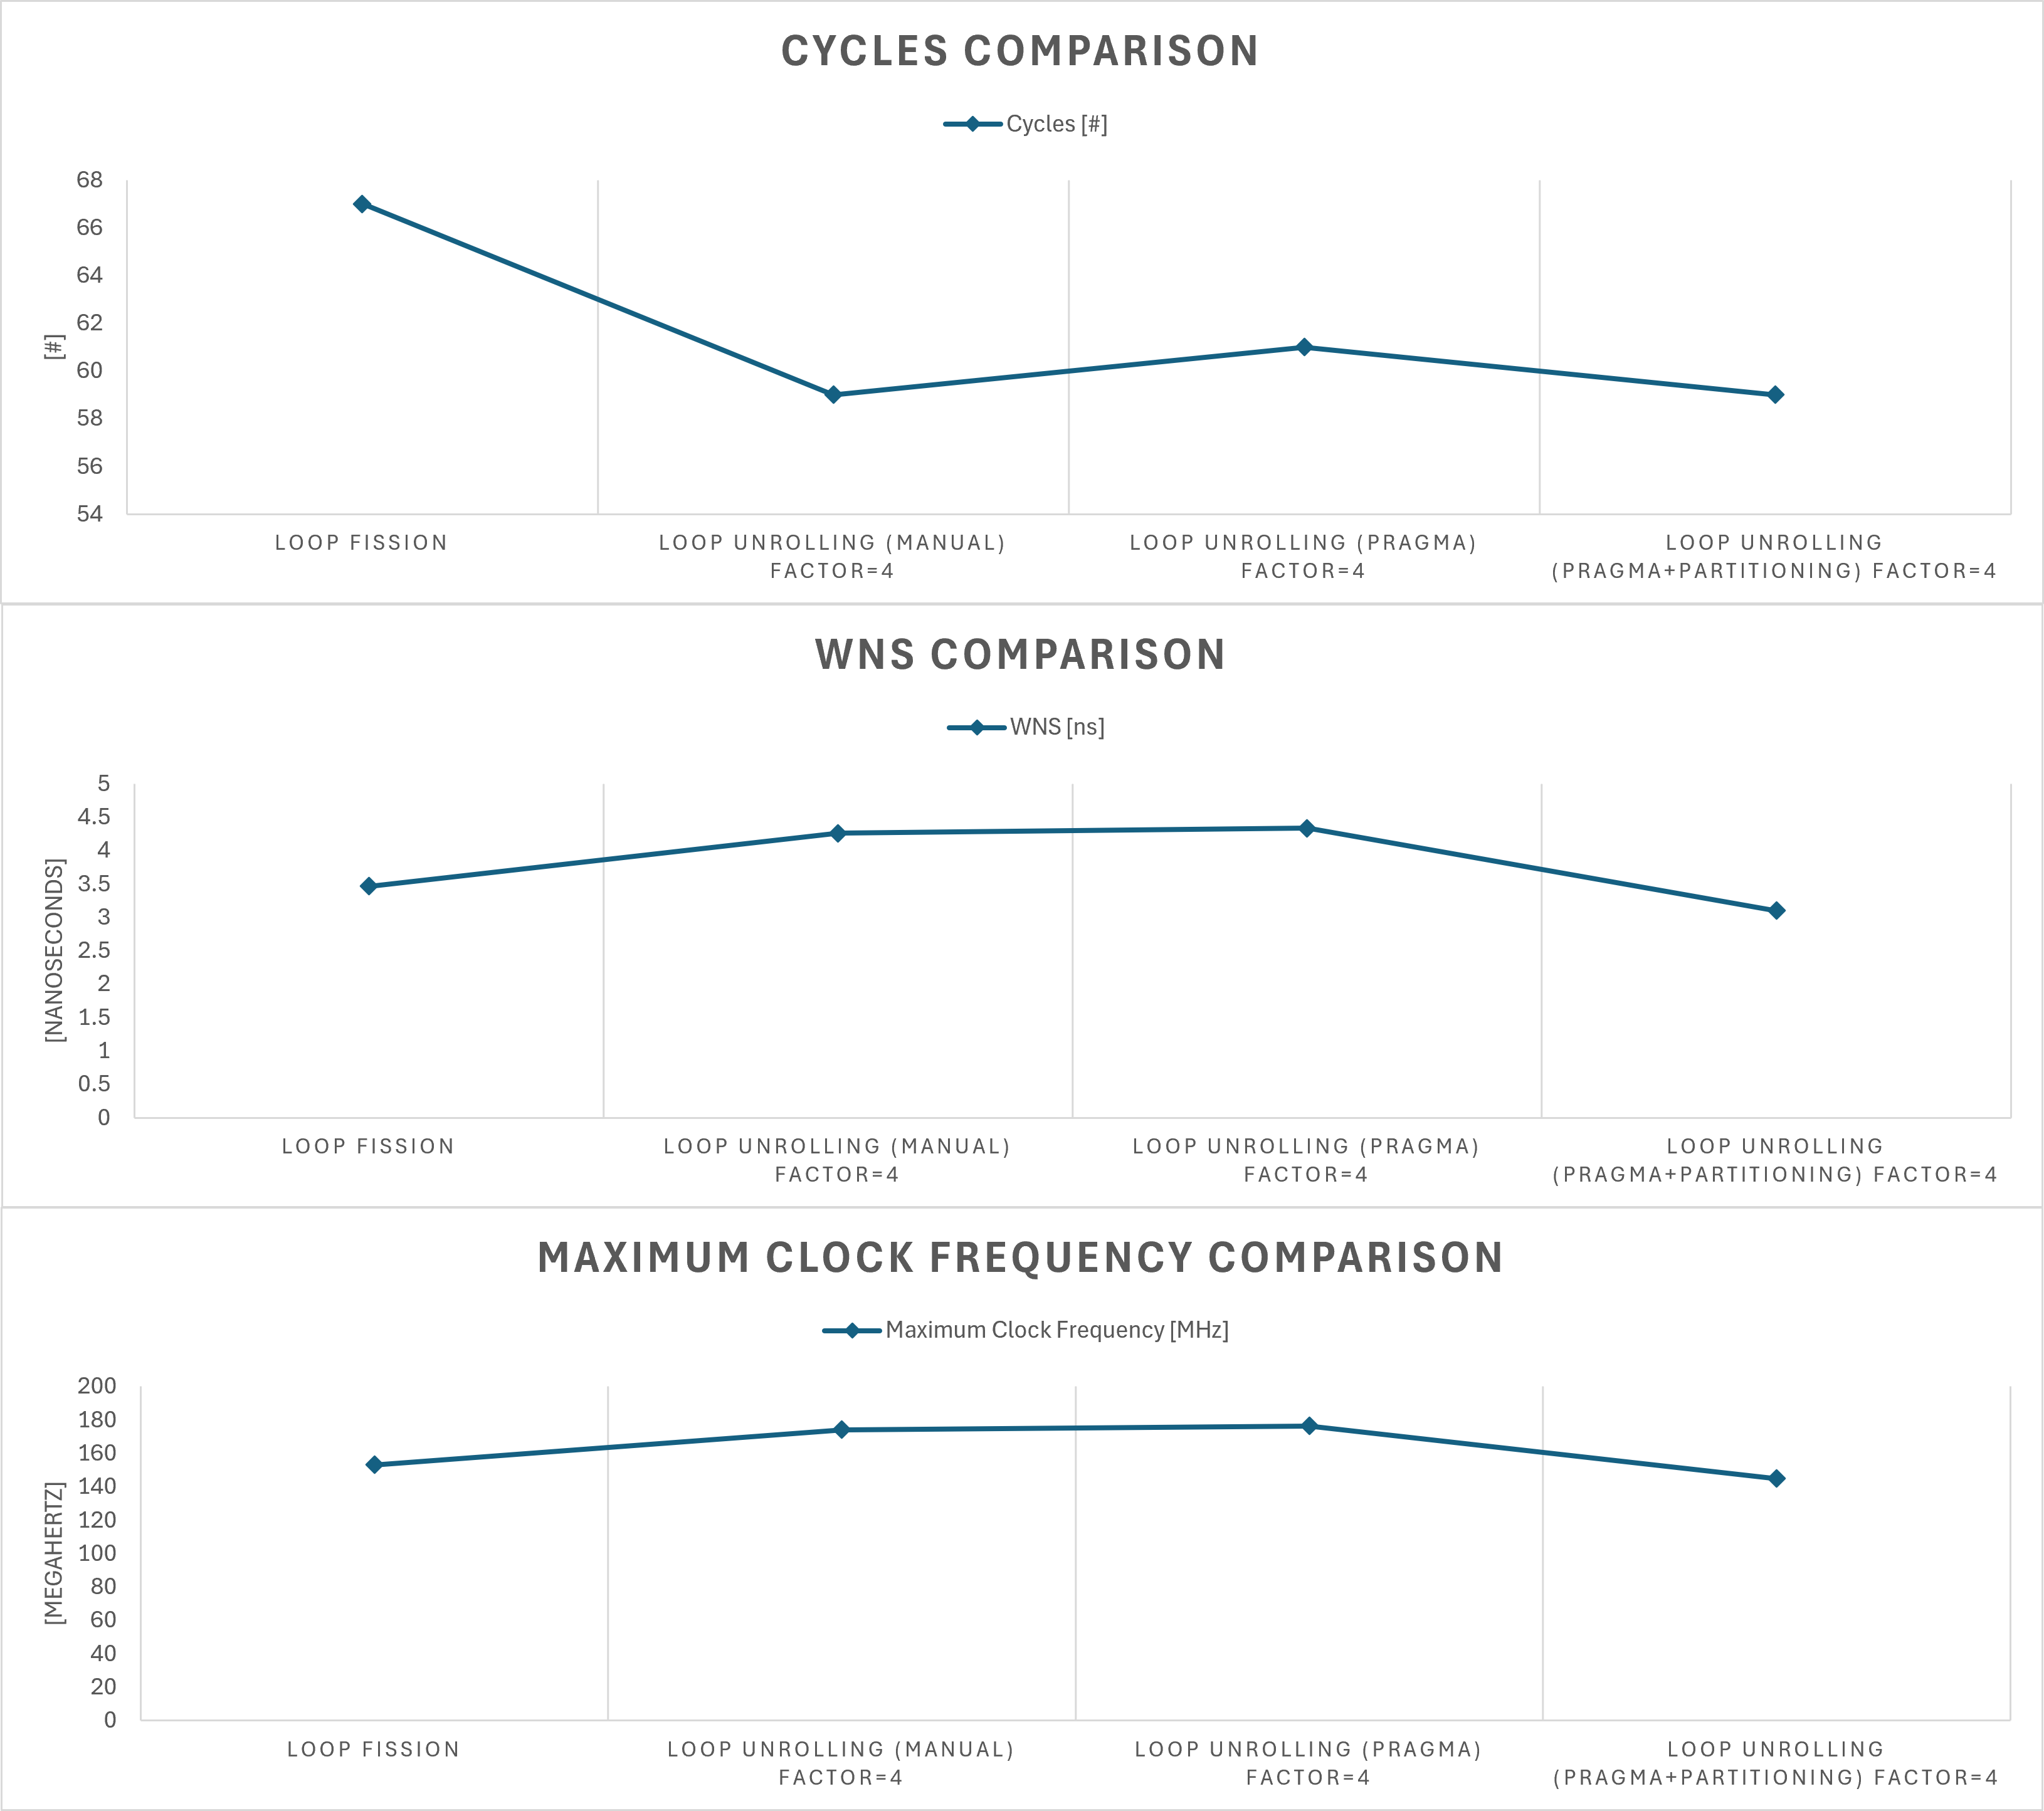
\includegraphics[width=0.8\textwidth]{solutions/loop_unrolling/factor4/loopunrollingfactor4timing.png}
    \caption{Vivado Loop Unrolling Factor=4 Timing Plot}
    \label{fig:vivado-loop-unrolling-factor4-solution-timing-plot}
\end{figure}

Analogamente all'unrolling di fattore pari a 2, anche in questo caso in corrispondenza della soluzione hardware basata su unrolling e partizionamento si ha un notevole aumento del contributo di potenza dinamica relativo al \textit{Clocks} comportando un aumento della potenza dinamica totale. 

\begin{table}[H]
    \centering
    \begin{tabular}{|c|c|c|c|c|c|c|c|}
        \hline
        \textbf{Solution} & \textbf{BRAM} & \textbf{Clock} & \textbf{Clocks} & \textbf{DSP} & \textbf{Logic} & \textbf{Set/}& \textbf{Data} \\
        & & \textbf{Enable} & & & & \textbf{Reset} & \\
        \hline
        Manuale & 1.32976193 & 0.382625905 & 0.253616716 & 0.921033497 & 0.543549308 & 0.010887122 & 0.585376518 \\
        \hline
        Automatico & 1.23103871 & 0.106978332 & 0.972227077 & 0.247065967 & 0.258892891 & 0.002585625 & 0.41881192 \\
        \hline
        Automatico & & & & & & & \\
        con & 0 & 0.328624592 & 2.560390625 & 0.298048515 & 1.146363211 & 0.0030065 & 1.324957004 \\
        Partitioning & & & & & & & \\
        \hline
    \end{tabular}
    \caption{Vivado Loop Unrolling Factor=4 Solution Dynamic Power Report [mW]}
    \label{tab:vivado-loop-unrolling-factor4-solution-dynamic-power-reproot}
\end{table}

\begin{table}[H]
    \centering
    \begin{minipage}[t]{0.45\linewidth}
        \centering
        \begin{tabular}{|c|c|}
            \hline
            \textbf{Solution} & \textbf{Dynamic Total} \\
            \hline
            Manuale & 4.026850996 \\
            \hline
            Automatico & 3.237600523 \\
            \hline
            Automatico & 5.661390447 \\
            con Partitioning & \\
            \hline
        \end{tabular}
        \caption{Vivado Loop Unrolling Factor=4 Solution Dynamic Power Report [mW]}
        \label{tab:vivado-loop-unrolling-factor4-solution-dynamic-power-reproot}
    \end{minipage}
    \hfill
    \centering
    \begin{minipage}[t]{0.45\linewidth}
        \centering
        \begin{tabular}{|c|c|}
            \hline
            \textbf{Solution} & \textbf{Energy Single Operation} \\
            \hline
            Manuale & 40.26850996 \\
            \hline
            Automatico & 32.37600523 \\
            \hline
            Automatico & 56.61390447 \\
            con Partitioning & \\
            \hline
        \end{tabular}
        \caption{Vivado Loop Unrolling Factor=4 Solution Energy Single Operation Report [pJ]}
        \label{tab:vivado-loop-unrolling-factor4-solution-solution-energy-single-operation-reproot}
    \end{minipage}
\end{table}

Bisogna notare un aspetto molto interessante. La potenza dinamica totale e l'energia per singola operazione associata alla soluzione hardware basata su loop unrolling automatico di fattore pari a 4 risultano essere pressocché le medesime di quelle relative all'unrolling automatico di fattore pari a 2. Questo potrebbe essere dovuto a ottimizzazione effettuate dal tool tramite la direttiva proprietaria dell'unrolling.